
\chapter{LaTeX}
\label{cha:latex}

Emacs comes with a package for editing \TeX\xspace and \LaTeX\xspace files.
However, this package is extremely limited in its functionality.
A far better package called \keyword{\auctex} can help you write your papers efficiently.


\section{Installation}
\label{sec:installation}

Here is the link \url{https://www.gnu.org/software/auctex/download.html} to install AUC\TeX.


\section{Configuration}
\label{sec:configuration}


Here is my code for configuring Emacs to use \auctex{}:
\begin{lstlisting}
;;;;;;;;;;;;;;;;;;;;;;;;;;;;;;;;;;;;;;;;;;;;;;;;;;
;; AUCTEX
;;;;;;;;;;;;;;;;;;;;;;;;;;;;;;;;;;;;;;;;;;;;;;;;;;
;; Automatically save style information when saving the buffer.
;; AUCTEX will create the auto directory automatically.
(setq TeX-auto-save t)

;; Parse file after loading it if no style hook is found for it.
(setq TeX-parse-self t)

;; If you often use \include or \input, you should make AUCTEX aware of the multifile document structure.
(setq-default TeX-master nil)           ; Query for master file.

;; Automatically insert '$...$' in plain TEX files, and '\(...\)' in LaTEX files by pressing $
(add-hook 'plain-TeX-mode-hook
          (lambda () (set (make-local-variable 'TeX-electric-math)
                          (cons "$" "$"))))
(add-hook 'LaTeX-mode-hook
          (lambda () (set (make-local-variable 'TeX-electric-math)
                          (cons "\\(" "\\)"))))

;; If this option is on, just typing (, { or [ immediately
;; adds the corresponding right brace ')', '}' or ']'.  The
;; point is left after the opening brace. If there is an
;; active region, braces are put around it.
(setq LaTeX-electric-left-right-brace t)

;; Get a full featuered LaTeX-section command.
(setq LaTeX-section-hook
      '(LaTeX-section-heading
        LaTeX-section-title
        LaTeX-section-toc
        LaTeX-section-section
        LaTeX-section-label))

;; Enable LaTeX Math mode by default.
;; Easy insertion of LaTeX math symbols.  If you give a
;; prefix argument, the symbols will be surrounded by dollar signs.
(add-hook 'LaTeX-mode-hook #'LaTeX-math-mode)

;; Define the function used when you type Enter.
(setq TeX-newline-function 'reindent-then-newline-and-indent)

;; When point is on one of the characters, it'll be unprettified automatically,
;; meaning you see the verbatim text again.
(setq prettify-symbols-unprettify-at-point 'right-edge)

;; Enable prettification in AUCTEX.
(add-hook 'LaTeX-mode-hook 'prettify-symbols-mode)

;; Add XeLaTeX program to run on the master or region file.
(eval-after-load "tex"
  '(add-to-list 'TeX-command-list
                '("XeLaTeX" "xelatex %s" TeX-run-command t t :help "Run xelatex")
                t))

;; Set the default command to run in LaTeX mode.
 (add-hook 'LaTeX-mode-hook (lambda ()
                              (setq TeX-command-default "XeLaTeX")))

;; ;; Add user defined viewer Skim.
(setq TeX-view-program-list '(("Skim" "/Applications/Skim.app/Contents/SharedSupport/displayline -g -b %n %o %b")))

;; Select the viewer to start view pdf output.
(setq TeX-view-program-selection
      '((output-dvi "open")
        (output-pdf "Skim")
        (output-html "open")))

;; Add TeX-source-correlate-mode to LaTeX mode to support forward 
;; and inverse search.
(add-hook 'LaTeX-mode-hook 'TeX-source-correlate-mode)

;; Whether Emacs retains the focus when viewing PDF files with Evince.
;; If this option is set to non-nil, Emacs will retain the focus.
;;(setq TeX-view-evince-keep-focus t)

;; If TeX-source-correlate-mode is active and a viewer is invoked,
;; the default behavior is to ask if a server process should be started.
;; Set this variable to t if the question should be inhibited and the
;; server should always be started.
(setq TeX-source-correlate-start-server t)

;; Make special mouse event do forward search at the clicked position.
(eval-after-load "tex"
  '(define-key TeX-source-correlate-map [C-down-mouse-1]
     #'TeX-view-mouse))

;; A function that will be called after performing an inverse search
;; from pdf in order to raise the current Emacs frame.
(setq TeX-raise-frame-function #'x-focus-frame)

;; When this boolean variable is non-nil, the error overview will be
;; automatically opened after running TEX if there are errors or warnings to show.
(setq TeX-error-overview-open-after-TeX-run t)

;; Get in-buffer notation for syntax error.
(add-hook 'LaTeX-mode-hook #'flymake-mode)

;; The output files will be placed in `build` directory.
;; This can improve the readability of the tex files.
;;(setq-default TeX-output-dir "build")

;; Add flyspell mode to latex mode.
(add-hook 'LaTeX-mode-hook 'flyspell-mode)

;; Add visual-line-mode to latex mode.
(add-hook 'LaTeX-mode-hook 'visual-line-mode)

;; Minor mode with distinct support for \label, \ref and \cite in LaTeX.
(add-hook 'LaTeX-mode-hook 'turn-on-reftex)
(setq reftex-plug-into-AUCTeX t)

;; If non-nil, insert braces after typing '^' and '_' in math mode.
(setq TeX-electric-sub-and-superscript t)

;; Support folding sections in LaTeX.
(add-hook 'LaTeX-mode-hook 'outline-minor-mode)
\end{lstlisting}


\subsection{Skim}
\label{sec:skim}

You should configure Skim to load automatically and let it know Emacs to locate the cursor.

The configuration is shown in Figure \ref{fig:skim-config}
\begin{figure}[!htbp]
  \centering
  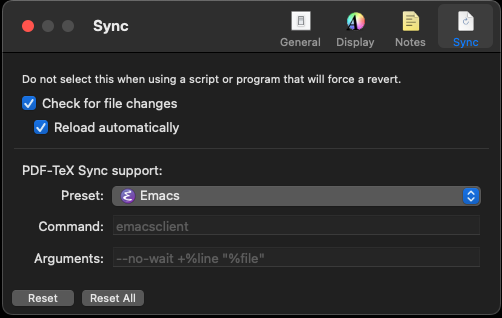
\includegraphics[width=0.8\textwidth]{skim}
  \caption{Skim configuration}
  \label{fig:skim-config}
\end{figure}

To display the TeX source line corresponding to a point in the PDF document, hold down the Shift and Apple key and click on a point in the PDF document.

\section[Basic Commands]{AUCTEX Commands}
\begin{center}
  \begin{longtable}[H]{l>{\bfseries}lp{0.5\textwidth}}

    \toprule
    \head{Group} & \head{Binding} & \head{Meaning}\\
    \midrule
    \endfirsthead

    \toprule
    \head{Group} & \head{Binding} & \head{Meaning}\\
    \midrule
    \endhead

    
    \midrule
    \multicolumn{3}{c}{{Continued on next page}}\\
    \bottomrule
    \endfoot{}

    \endlastfoot

    
    \multirow{3}{*}{insert} & C-c C-s & insert section macros\\
                 & C-c C-e & insert environment, with \keyword{C-u} prefix will change the current environment\\
                 & C-c C-m & insert \LaTeX\xspace macro\\
    \midrule
    \multirow{3}{*}{comment} & M-; & insert comment, if there is a region, comment or comment the region\\
                 & C-c ; & comment or uncomment the current region\\
                 & C-c \% & command or uncomment current paragraph\\
    \midrule
    \multirow{6}{*}{run} & C-c C-c & run command on the current document\\
                 & C-c C-a & compile the document until it is ready and then run the viewer\\
                 & C-c C-r & run on region(also use preamble)\\
                 & C-c C-b & run only on current buffer(\lstinline[language=TeX]|\include| or \lstinline|\input|), using the preamble from the master file\\
                 & C-c C-k & kill running process\\
                 & C-c C-v & start a viewer without confirmation\\
    \midrule
    \multirow{3}{*}{debug} & C-c \textasciigrave{} & find the next error in the TeX output buffer\\
                 & C-c C-l & display output so that most recent output can be seen\\
                 & M-g p & find the previous error in the TeX output buffer\\
    \midrule
    \multirow{3}{*}{move} & C-M-a & move point to the beginning of current environment\\
                 & C-M-e & move point to the end of current environment\\
                 & C-c \textbackslash{} & go the 'master' file in the document associated with the current buffer\\
    \midrule
    \multirow{10}{*}{reftex} & C-c \& & view cross reference of macro at point\\
                 & C-c ( & insert a unique label\\
                 & C-c ) & make a LaTeX reference\\
                 & C-c - & display the TOC window and highlight line corresponding to current position\\
                 & C-c / & put selection or the word near point into the default index macro\\
                 & C-c < & query for an index macro and insert it along with its arguments\\
                 & C-c > & display a buffer with an index compiled from the current document\\
                 & C-c [ & make a citation using BibTeX database files\\
                 & C-c \textbackslash{} & add current selection or word at point to the phrases buffer\\
                 & C-c \textbar{} & switch to the phrases buffer, initialize if empty\\
    \midrule
    \multirow{7}{*}{outline} & C-c @ C-t & hide all of buffer except headings\\
                 & C-c @ C-a & show all of the text in the buffer\\
                 & C-c @ C-q & hide everything but top levels headers\\
                 & C-c @ TAB & show all direct subheadings of this heading\\
                 & C-c @ C-k & show all subheadings, but not bodies\\
                 & C-c @ C-p & go to previous visible heading\\
                 & C-c @ C-n & go to next visible heading\\
    \midrule
    \multirow{3}{*}{narrow} & C-x n e & make text outside environment invisible\\
                 & C-x n n & make text outside region invisible\\
                 & C-x n w & un-narrow\\
    \midrule
    \multirow{5}{*}{toggle} & C-c C-t C-p & toggle between DVI and PDF output\\
                 & C-c C-t C-i & toggle interactive mode\\
                 & C-c C-t C-s & toggle Sync\TeX(or source specials) support\\
                 & C-c C-t C-o & toggle useage of Omega/lambda\\
                 & C-c C-t C-w & toggle whther AUCTEX should stop at warnings as well as errors\\

    doc & C-c ? & get documentation about the packages installed on your system, using texdoc to find the manuals\\
    \midrule
    \multirow{2}{*}{mark} & C-c . & mark current environment\\
                 & C-c * & mark current section\\
    \bottomrule
    \caption{Basic commands for editing \TeX\xspace{} files}
    \label{tab:basic-commands}
  \end{longtable}
\end{center}


If you enable braces auto completion, using \keyword{C-q} before typing (, \{ or [ will suppress it.


\keyword{C-c c-s} run \lstinline[language=TeX]|LaTeX-section arg| to insert a section.
The argument \argument{arg} determines the type of section to be inserted:
\begin{itemize}
\item If \argument{arg} is nil or missing, use the current level.
\item If \argument{arg} is a list (selected by \keyword{C-u}), go downward one level.
\item If \argument{arg} is negative, go up that many levels.
\item If \argument{arg} is positive or zero, use absolute level:
  \begin{itemize}[label=$\maltese$]
  \item + 0 : part
  \item + 1 : chapter
  \item + 2 : section
  \item + 3 : subsection
  \item + 4 : subsubsection
  \item + 5 : paragraph
  \item + 6 : subparagraph
  \end{itemize}
\end{itemize}


TeX-error-overview Show an overview of the errors and warnings occurred in the last TEX run.


Running TEX or LaTEX will only find regular errors in the document, not examples of bad style.
Furthermore, description of the errors may often be confusing.
The utilities \argument{lacheck} and \argument{chktex} can be used to find style errors, such as forgetting to escape the space after an abbreviation or using '...' instead of '\ldots' and other similar problems.
You start \argument{lacheck} with \keyword{C-c C-c Check RET} and \argument{chktex} with \keyword{C-c C-c ChkTeX RET}.
The result will be a list of errors in the \argument{'*compilation*'} buffer.
You can go through the errors with \keyword{C-x \textasciigrave{}}, which will move point to the location of the next error.





%%% Local Variables:
%%% mode: latex
%%% TeX-master: "emacs"
%%% End:
